\chapter{Social Routing Client Application}
The Social Routing Client is composed by four major components, each with it's own compromise and objective.
The Activities/Fragments[TODO REF] to represent the User Interface (UI) where the user can interact with, the ViewModels[TODO REF] to store
and manage UI-related data, a Repository[TODO REF] to handles data operations and knows where to get the data from and a 
Remote Data Source[TODO REF] to communicate with external components, for instance Social Routing API and Google API'S[TODO REF]. 
This logic is represented in Figure [TODO FIG]

\begin{figure}[h]            
        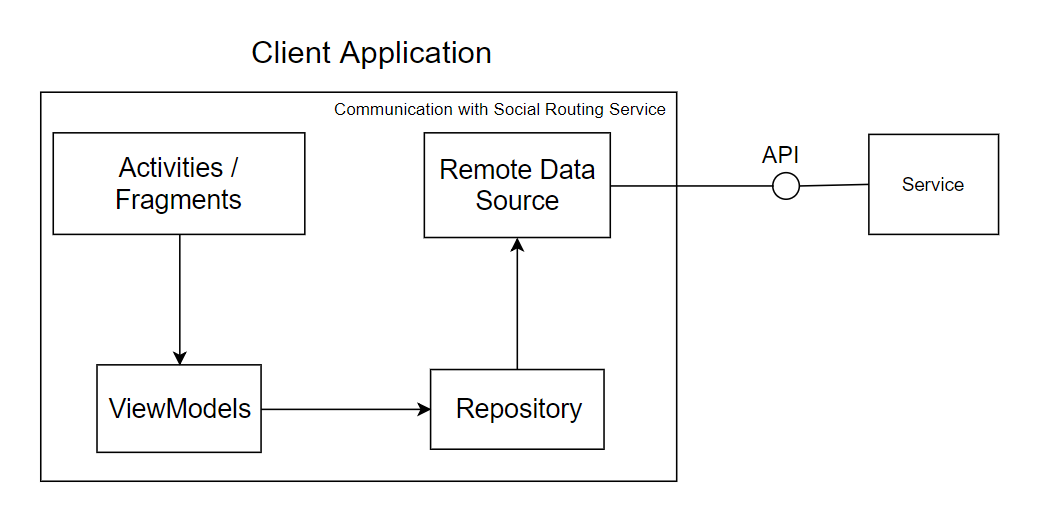
\includegraphics[width=\textwidth]{images/project-structure/social-routing-client-application-structure.PNG}
        \caption{Social Routing Client architecture.}
\end{figure}

\section*{Activities/Fragments}
The concern of this component is to represent the user the Application flow, where the user can navigate and interact with.
All activities extend of a BaseActivity that as a global behaviour, like when the data was changed is necessary to reformulate the view to the user see the 
information updated. \\

Each Activity has its own :
\begin{itemize}
        \item Design: defined by one or more layouts that contains buttons, images, input text, fragments (for instance the map fragment provided by Google), where the user can interact.
        \item Behaviour: when de data is changed the view need to be reformulated, and this behaviour is defined with a success behaviour and a Error behaviour, using the ViewModel.
\end{itemize}

A example activity is the NavigationActivity where the user can navigate to all the functionalities of the application, after google authentication, like the creation of a route, 
search by routes and the user profile. This activity as a left panel where you can navigate to other activities with different purposes like the route creation and the user profile, 
however the activity it self has the search functionality, where you can input text like the location name that is pretended and a button to navigate to the activity that shows the 
results of that search.

\section*{ViewModels}
Component used when the UI experiences a change, the ViewModel calls
other components to load the data, and it can forward user requests to
modify the data, however the ViewModel doesn't know about UI components, 
it is completely separated from them. \\
This component has a simple implementation, the application contains two ViewModels one for the Routes information (get, creation, update, search) and the other 
to the User (get, delete). It uses the repository to obtain the data and then return it in the shape of Livedata[TODO REF].

\section*{Repository}
The Repository Handles data operations, knows where to get the data from
and what API calls to make when data is updated. A repository can be
considered to be a mediator between different data sources, such as web services. \\
The application has a repository specified to the Social Routing API and another to Google Maps API. Each one as correspondent Web Service that uses the
framework Retrofit[TODO REF], used to make a synchronous or asynchronous HTTP request to the remote webserver. The Repository obtains the data
from the web server and only have to possible request status Failure and Success and returns the data contained in a LiveData, because when the data suffers
and update it could be observable. \\
The Repository specified to our API (Social Routing API) knows all the endpoints that should make the request, depending on the objective and the functionality, like 
the endpoints to sign in, to get user info, routes, create a route, get all categories, update a route, etc... \\
On the other hand the, the other repository is used to make request to the Google Webserver (Google Maps API) about the geocode of a location and the directions to a coordinate in the map. 

\section*{Remote Data Source}
Module that has the objective of communicating with external APIs and it communicates by doing requests to the Social Routing API and the Google Maps API. 
The Component knows the structure of the HTTP request to the endpoints, like the parameters and meta-data necessary to obtain the required Response.
After the request done, the webservers provide the response with Json[TODO REF] format, however the response is deserialized using the library Jackson[TODO REF],
to convert it to Object. So was defined all the input model objects, to automatically deserialize the response to object.\\

The Client Application has the minimum API level 19 and the target API level is 28, so the Platform version is the Android 9.
It uses the Kotlin as unique the programming language in the project, is a object oriented programming language and is getting more and more used nowadays. 
The goal was to improve the coding experience in a way that was practical and effectual. Kotlin is entirely compatible with Java and was specifically designed
to improve existing Java models by offering solutions to API design deficiencies. \\
The core functionalities of the application require a map to create the routes and to show them, the way that was done was using the Google Maps, setting up the 
Google Play Services to the project.\\
All the functionalities of the application are provided from de Social Routing Server, except all that is related to the Google Maps. All the information is required from the server doing
requests to the correspondent endpoint and is always necessary send the token created by the server, except when is the authentication request that is needed to send to the server the idToken
provided from the Google Account. The request that are related to obtain locations or to the Map is necessary to make a specific request to the Google Maps API. \\
As an example, the user first experience flow of the application is the following:
        \begin{itemize}
                \item The first screen is the user authentication with the backend server using the google account.
                \item The user will be redirected to a navigation screen that contains a routes search bar and a left panel with buttons to redirect to the screens of user profile and route creation.
                \item After the user search routes using a location, will be redirect to a new screen, that obtains a list of routes.
                \item After clicked in a route, the user will be redirect to a screen that shows the map, the route in it and a button to start Live Tracking.
                \item The user starts Live Tracking is showed the optimal way to the route.
                \item The user wants to see the his profile, so he may go back until the navigation screen and click in the left panel and then in the User Profile button.
                \item Is showed the user information (user rating, name, email and routes created).
                \item Then the user wants to create a route, go back to Navigation screen again and click in the button Route Creation.
                \item Is redirected to a new screen that shows the map, a button to finish and a form, asking the location of the route that will be created.
                \item User inserts the location and the map zoom in into the chosen location.
                \item The User clicks in the map to select the path of the route, if something wrong the user can delete the last point of the route clicking the button on the top of the screen.
                \item When finished the user click in the button to fill the final form that contains the name, description and category of the route.
        \end{itemize}